\chapter{Scoping}\label{ch:scoping}

\section{Profilo della software house}\label{sec:profilo-della-software-house}
Atedeg è una software house che opera sul territorio cesenate. È composta da un team piuttosto affiatato di 10 persone dalle competenze più variegate, che si occupano di sviluppo software.

Il core team è composto da Giacomo, Linda, Nicolas e Nicolò, quattro amici che si sono conosciuti all'università e hanno deciso, una volta terminati gli studi, di fondare la software house.
Nel corso degli anni, il team si è arricchito di nuovi membri, che hanno portato con sé nuove idee e hanno contribuito a mantenere Atedeg un ambiente dinamico aperto all'innovazione.

Essendo una piccola software house, Atedeg non adotta una rigida suddivisione gerarchica dei ruoli. In particolare, non esiste un senior management che decida quali progetti intraprendere o meno: infatti, tali decisioni vengono prese in comune dai membri del team, che si riuniscono periodicamente per discutere di nuovi possibili progetti. In questo modo, tutti i colleghi hanno la possibilità di esprimere le proprie opinioni e di partecipare attivamente alla vita dell'azienda.

All'interno di Atedeg si dà molta importanza all'arricchimento personale e professionale, e si cerca di dare a tutti gli sviluppatori la possibilità di crescere e di migliorare le proprie competenze. Per questo motivo sono incentivati lo studio e la formazione e, qualora i dipendenti ne facciano richiesta, l'azienda cerca di finanziare la loro partecipazione a conferenze di calibro internazionale.
In particolare, Linda ha avuto modo di assistere al ciclo di conferenze \href{https://dddeurope.com}{\emph{Domain Driven Design Europe}} del 2019 e da quel momento ha cercato di introdurre gradualmente nell'azienda il Domain Driven Design, che è stato adottato in due progetti conclusi con successo.

\section{Profilo del committente}\label{sec:profilo-del-committente}
Mambelli è un caseificio di Cesena a gestione familiare che si occupa di produzione e vendita di prodotti caseari. L'azienda è stata fondata nel 1972 e nel corso degli anni si è arricchita di nuove produzioni ricevendo anche diversi riconoscimenti come il premio \emph{Italian Cheese Award}.
Grazie alla crescente popolarità è aumentata anche la domanda di prodotti e, per poterla soddisfare, Mambelli ha deciso di migliorare il proprio sistema informativo automatizzando i diversi processi aziendali laddove possibile.

Il nuovo sistema deve essere pronto entro il 30 settembre per poter essere utilizzato appieno nella gestione del grande flusso di ordini che si verifica intorno al periodo natalizio. Quindi il portale di e-commerce con la possibilità di effettuare automaticamente nuovi ordini rappresenta un \emph{Minimum Viable Product} (MVP) la cui consegna entro i tempi prestabiliti determina la buona riuscita o meno del progetto.

L'azienda è gestita da Raffaella che si occupa dell'acquisto delle materie prime e della pianificazione della produzione dei formaggi. Il marito di Raffaella, Gianluca, si occupa invece dei rapporti coi clienti e della gestione degli ordini. Inoltre il caseificio assume due casari che si occupano della produzione dei formaggi e del controllo qualità dei prodotti. Infine l'azienda ha diversi dipendenti impiegati nel settore della logistica.

\section{Richiesta del committente}\label{sec:richiesta-del-committente}
L'attuale sistema informativo adottato dal caseificio Mambelli risulta inadeguato per poter gestire l'aumento nella domanda dei prodotti: molti dei processi aziendali sono infatti gestiti manualmente o su semplici fogli elettronici. In particolare, i problemi che il caseificio vorrebbe risolvere sono i seguenti:
\begin{itemize}
  \item \textbf{Gestione degli ordini:} al momento tutti gli ordini arrivano tramite mail o, in maniera informale, tramite comunicazioni telefoniche. Gianluca impiega quindi molto tempo per raccoglierli e inserirli nel sistema informativo. Inoltre, non essendo strutturati, gli ordini non sono facilmente consultabili e non è possibile ricavare informazioni utili per la pianificazione della produzione
  \item \textbf{Pianificazione della produzione:} la pianificazione di quali prodotti mandare in produzione viene fatta manualmente da Raffaella sulla base della sua grande esperienza nel campo. Per prendere queste decisioni Raffaella consulta un foglio elettronico che riporta alcune informazioni sugli ordini passati e su quanto è stato prodotto in precedenza. Sebbene questo metodo sia sufficiente per poter effettuare la programmazione, presenta due importanti problemi:
        \begin{itemize}
          \item Raffaella, grazie alla sua esperienza, è l'unica in grado di pianificare la produzione; se dovesse essere assente per qualche motivo, la produzione non potrebbe essere pianificata in maniera adeguata
          \item Sebbene l'esperienza di Raffaella sia sufficiente per avere delle buone pianificazioni, queste potrebbero essere ottimizzate ulteriormente con il supporto di sistemi informativi più avanzati riducendo i tempi morti nell'uso dei macchinari e minimizzando gli sprechi di materie prime
        \end{itemize}
  \item \textbf{Integrazione con sistemi preesistenti:} il caseificio Mambelli utilizza altri moduli software per gestire la tracciabilità dei prodotti e lo stoccaggio delle merci; per questo motivo è fondamentale che qualunque sistema realizzato possa essere integrato con questi sistemi
\end{itemize}

\section{Project Scoping Meeting}
\label{sec:project-scoping-meeting}

Il team di Atedeg ha valutato se prendere in considerazione o meno la proposta fatta dal caseificio. Dalla descrizione dei bisogni del committente riportata alla sezione precedente, emerge come il dominio del problema sia piuttosto ampio: infatti sarebbe richiesta la realizzazione di un sistema per la gestione degli ordini dei clienti che si possa integrare con altri sistemi eventualmente adottati. Inoltre, il secondo punto delle richieste potrebbe necessitare la realizzazione di un sistema di supporto alle decisioni con una profonda conoscenza del dominio del caseificio.
Linda propone quindi di effettuare una prima riunione con il committente per discutere la proposta adottando una metodologia improntata sul Domain Driven Design; infatti, questo approccio risulta ideale per domini aziendali simili ed è già stato utilizzato con successo dal team.

\subsection{Prima riunione}
\label{sec:prima-riunione}
Lo scopo della prima riunione è stato quello di discutere la proposta del committente e permettere al core team del progetto di conoscere il dominio del caseificio. Il committente ha messo a disposizione la propria sala riunioni per tre ore per svolgere il primo incontro.
Su suggerimento di Linda, si è deciso di adottare la tecnica dell'\emph{Event Storming}~\cite{cit:event-storming} per condurre la riunione.

\subsubsection{Partecipanti}
\label{sec:prima-riunione-partecipanti}
\begin{itemize}
  \item Linda (facilitatore)
  \item Giacomo, Nicolò e Nicolas (membri del core team)
  \item Raffaella (proprietaria del caseificio e responsabile pianificazione)
  \item Gianluca (responsabile ordini e addetto vendite)
  \item Simone (casaro e responsabile produzione)
  \item Luisa (responsabile magazzino)
\end{itemize}

\subsubsection{Setup}
\label{sec:prima-riunione-setup}
Sebbene il committente abbia fornito la sala riunioni per tutta la mattinata (dalle 9:00 alle 12:00) il team ha segnato le 9:30 come orario di inizio effettivo per avere il tempo di preparare in maniera opportuna la sala.
Infatti, questa presenta la classica disposizione con un grande tavolo al centro circondato da sedie. Secondo Brandolini, padre dell'Event Storming, questo è un ``anti pattern'': infatti, porta i partecipanti a pensare che il meeting si svolgerà come tutte le altre (noiose) riunioni aziendali dove una persona parla e gli altri stanno seduti ad ascoltare~\cite[pp.~116-118]{cit:event-storming-book}.

L'approccio dell'Event Storming vuole puntare su una forte interazione fra i diversi esperti dei settori aziendali per approfondire la conoscenza del dominio e allo stesso tempo far emergere i veri bisogni del cliente. Per ottenere questo risultato si organizza la riunione in modo da sorprendere i partecipanti incentivandoli a una partecipazione attiva.

È stato appeso un grande rotolo di carta lungo tutta una parete della sala e sono stati messi a disposizione numerosi blocchetti di post-it colorati e pennarelli come mostrato in \Cref{fig:event-storming-setup}. Inoltre, il grande tavolo è stato spostato dal centro della stanza e le sedie sono state impilate per scoraggiare che i partecipanti si siedano durante la riunione diventando degli osservatori passivi.

\begin{figure}[!ht]
  \centering
  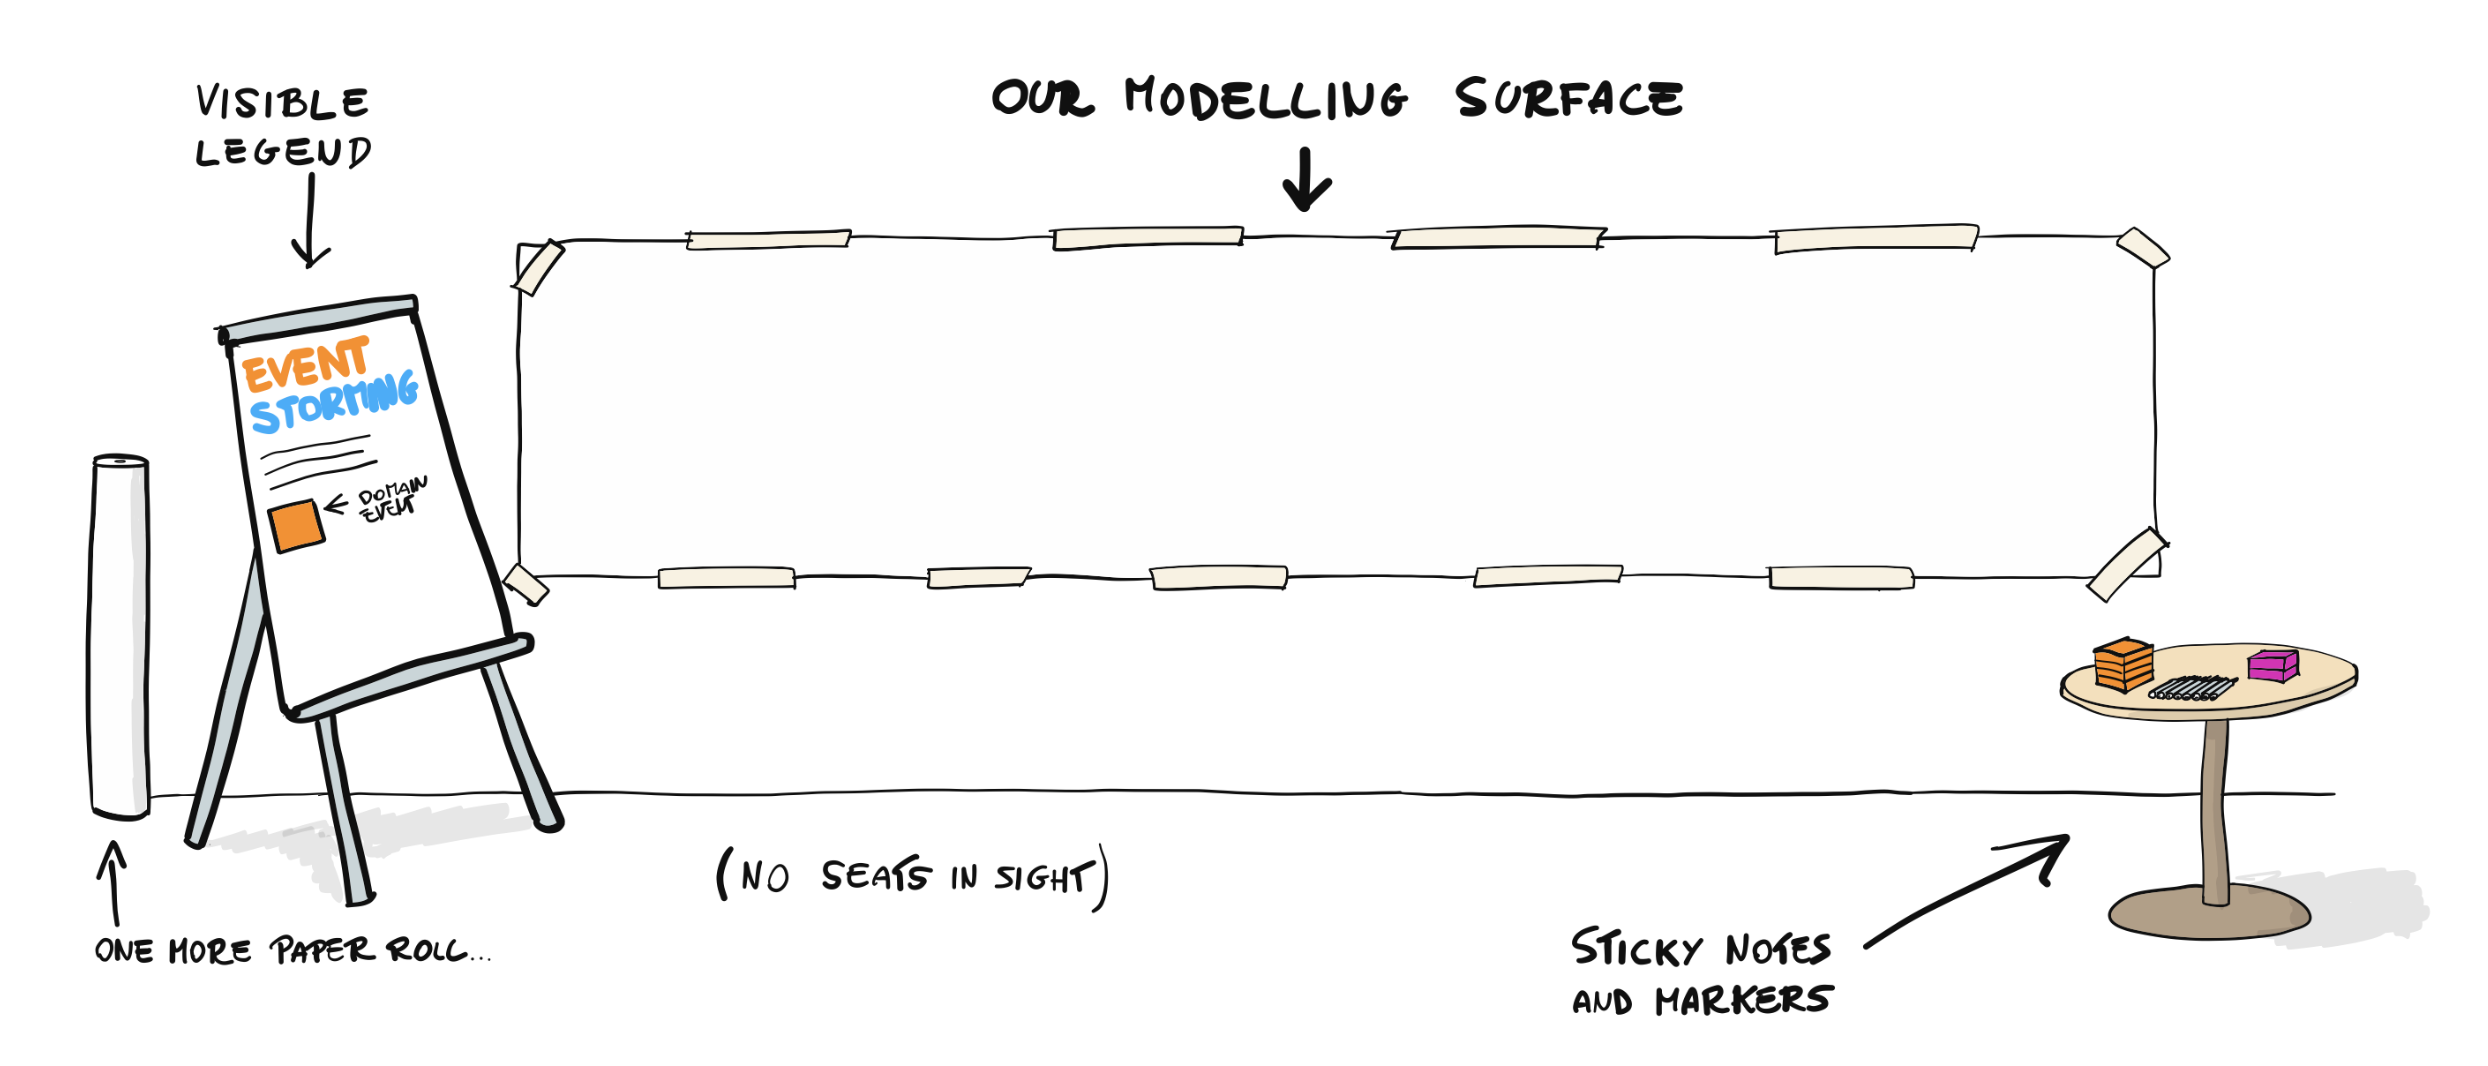
\includegraphics[width=0.8\textwidth]{images/event-storming-setup.png}
  \caption{Preparazione per una sessione di Event Storming}
  \label{fig:event-storming-setup}
\end{figure}

\subsubsection{Kick off}
\label{sec:prima-riunione-kick-off}
Intorno alle 9:30 è iniziata la riunione; si poteva notare che i partecipanti erano spaesati ma allo stesso tempo incuriositi dal grande rotolo di carta.
Linda, nel ruolo di facilitatore, ha lanciato il meeting con un breve giro di presentazioni.
Successivamente, ha spiegato in maniera esplicita l'obiettivo della riunione in modo che fosse chiaro a tutti i partecipanti.

\begin{tabularx}{.9\textwidth}{rX}
  \speak{Linda} & L'obiettivo di questo incontro è analizzare gli attuali processi aziendali del caseificio per cercare di capire come possano essere migliorati e automatizzati, interagendo armonicamente fra loro e con sistemi preesistenti. All'inizio il processo potrebbe sembrarvi difficile ma vi invito a intervenire senza paura, qualunque cosa facciate sarà utile. \\
\end{tabularx}

La spiegazione del facilitatore è volutamente molto breve: non si vuole annoiare con una lunga descrizione ma lasciare che gli esperti di dominio inizino subito a descrivere il loro lavoro. L'importante è che il facilitatore trasmetta una sensazione di sicurezza e disponibilità ad aiutare i partecipanti.

\begin{tabularx}{.9\textwidth}{rX}
  \speak{Linda}     & Vorrei che descriveste degli eventi rilevanti al vostro ambito aziendale su questi post-it arancioni e che li attacchiate in ordine cronologico sul rotolo di carta. \\
  \speak{Raffaella} & Potresti spiegare meglio cosa intendete con ``eventi''?                                                                                                              \\
  \speak{Linda}     & Certamente! Ti faccio un esempio concreto: lavoro nel settore degli ordini; un evento che mi interessa è quando ricevo via email un nuovo ordine.                    \\
                    & \emph{Mentre parla, Linda scrive la frase ``Nuovo ordine ricevuto per email'' su un post-it arancione}                                                               \\
  \speak{Raffaella} & Ah, adesso mi è chiaro... quindi un evento che mi interessa potrebbe essere ``Fatto nuovo piano di produzione''?                                                     \\
  \speak{Linda}     & Esatto! L'importante è che nel descrivere l'evento usiate sempre un verbo al passato come ha fatto adesso Raffaella.                                                 \\
\end{tabularx}

\subsubsection{Esplorazione caotica}
\label{sec:prima-riunione-esplorazione-caotica}

I primi minuti di una riunione di Event Storming sono sempre i più difficili: i partecipanti potrebbero essere spiazzati dalla nuova modalità di interazione e fare fatica a individuare degli eventi da scrivere sui post-it.
È fondamentale in momenti come questo che il facilitatore dia loro supporto ma non li guidi attivamente; nel caso in cui non sia presente una persona coraggiosa in grado di rompere il ghiaccio attaccando il primo post-it, potrebbe farlo il facilitatore con un esempio.
Fortunatamente, in questo caso Raffaella ha già chiaro cosa scrivere e attacca per prima un post-it alla parete.

\begin{tabularx}{.9\textwidth}{rX}
  \speak{Linda} & Ottimo, grazie Raffaella! Come vedete basta che scriviate eventi rilevanti per il settore aziendale dove lavorate. Non ci sono risposte sbagliate, scrivete tutto quello che vi viene in mente. \\
\end{tabularx}

Spesso potrebbero formarsi dei piccoli gruppetti di persone che si confrontano per scegliere il termine più adatto da scrivere sui post-it. È compito del facilitatore cercare di ``spezzare'' questi gruppetti per evitare che continue discussioni riducano il flusso di post-it e che non emergano elementi contraddittori fondamentali all'analisi del dominio.

Il modello inizia a prendere forma, il numero di post-it attaccati cresce rapidamente e i partecipanti si sentono sempre più a proprio agio. Potrebbero esserci diversi post-it duplicati o incongruenze; ciò è perfettamente normale, anzi non bisogna cercare la perfezione in questa fase.

\subsubsection{Controllo della coerenza del risultato}
\label{sec:prima-riunione-controllo-della-coerenza-del-risultato}

Quando il flusso di post-it inizia a diminuire ed emerge una timeline approssimata è il momento adatto per passare alla seconda fase. Il risultato ottenuto dalla prima fase, come mostrato in \Cref{fig:event-storming-exploration}, può presentare post-it duplicati e cluster all'interno di un flusso disorganizzato. Questo punto di partenza verrà rifinito in modo da far sì che venga rispettata correttamente la timeline del dominio e che possa emergere un modello coerente.

\begin{figure}[!ht]
  \centering
  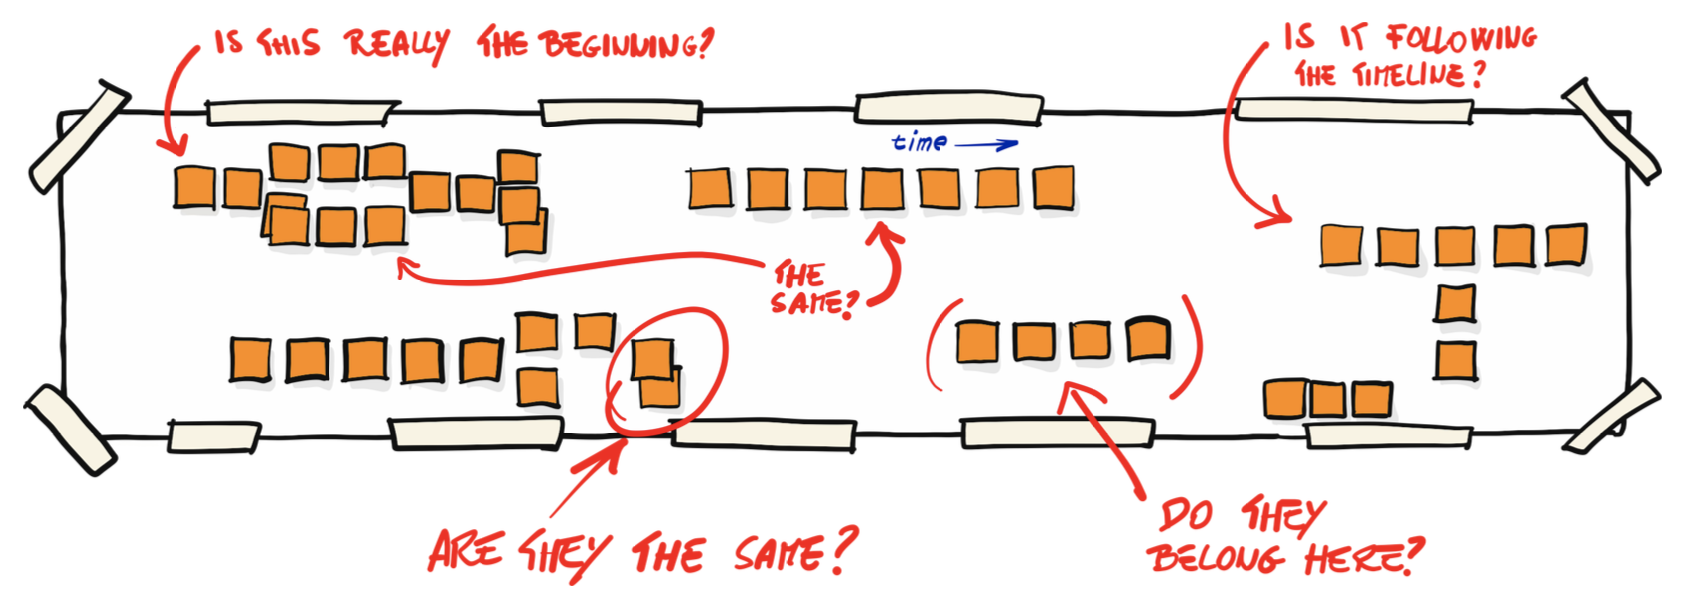
\includegraphics[width=0.8\textwidth]{images/event-storming-exploration.png}
  \caption{Esempio di come può apparire il modello ottenuto dalla prima fase di esplorazione caotica}
  \label{fig:event-storming-exploration}
\end{figure}

Per riordinare i vari cluster di eventi è utile individuare le cosiddette \emph{swimlanes}: suddivisioni logiche dei vari eventi raggruppandoli in base a omogeneità per attori o dipartimenti aziendali interessati. Un esempio è mostrato in \Cref{fig:event-storming-swimlanes}.

\begin{figure}[!ht]
  \centering
  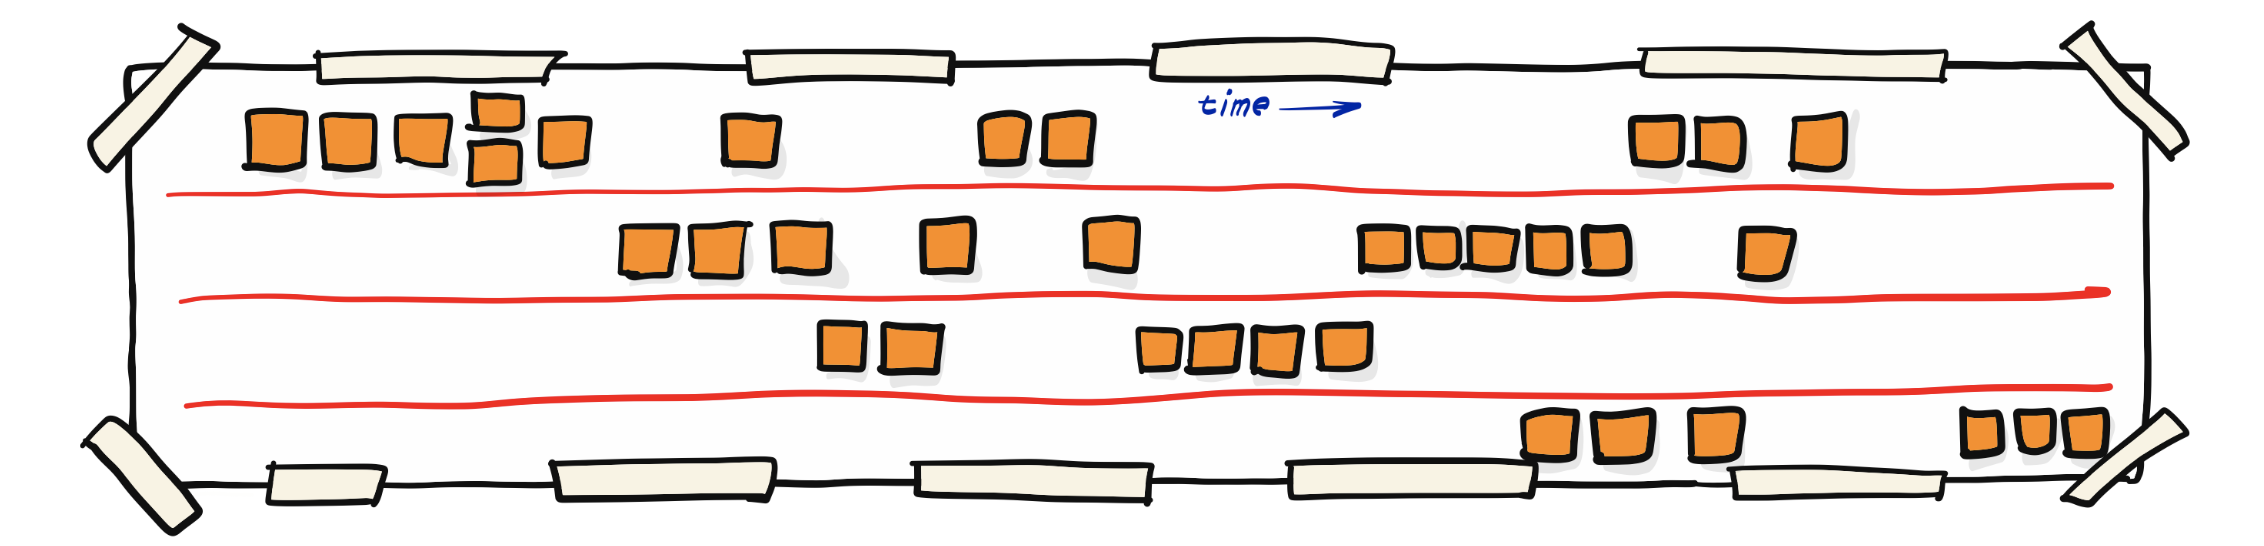
\includegraphics[width=0.8\textwidth]{images/event-storming-swimlanes.png}
  \caption{Esempio di individuazione di swimlanes}
  \label{fig:event-storming-swimlanes}
\end{figure}

Riordinare gli eventi in maniera coerente comporterà il confronto fra esperti di diversi settori aziendali; spesso potrebbero emergere delle incongruenze nel modo in cui i vari silos interpretano gli eventi. Queste discussioni sono fondamentali per individuare i punti dove sono presenti delle criticità nell'interazione fra i dipartimenti; il facilitatore non deve farsi sfuggire tali discussioni e marcare con appositi post-it viola i punti dove è necessario un ulteriore approfondimento.

\subsubsection{Persone e sistemi esterni}
\label{sec:prima-riunione-persone-e-sistemi-esterni}

Una volta che il modello è stato riordinato si possono inserire per ogni flusso di eventi le persone (o attori, per utilizzare la terminologia UML) che vi interagiscono.

\begin{tabularx}{.9\textwidth}{rX}
  \speak{Linda}    & Ora vi chiedo di indicare, per i flussi di eventi di vostra competenza, quali sono le persone che avviano tale flusso e che vi interagiscono.                                                  \\
                   & \emph{Nel mentre, Linda disegna su un post-it giallo una versione stilizzata di Raffaella con sotto scritto il suo nome e lo attacca all'inizio del flusso di pianificazione della produzione} \\
  \speak{Gianluca} & Quindi visto che io gestisco gli ordini dovrei mettermi all'inizio di quel flusso?                                                                                                             \\
  \speak{Linda}    & Esatto, potremmo metterci anche un generico ``cliente'' visto che è lui che fa partire effettivamente l'ordine e tutto il flusso che lo gestisce.                                              \\
\end{tabularx}

Una volta inserite le persone si può fare lo stesso in maniera analoga con i sistemi esterni con cui un flusso deve interagire.
Nel nostro caso, il sistema della tracciabilità è un sistema esterno:

\begin{tabularx}{.9\textwidth}{rX}
  \speak{Linda}    & Mi sembrava di avervi sentito discutere di un sistema della tracciabilità che usate per i vostri prodotti.                                                                                                        \\
  \speak{Gianluca} & Sì, è un sistema esterno che dobbiamo utilizzare per garantire la tracciabilità in caso ci siano problemi con dei lotti.                                                                                          \\
  \speak{Linda}    & Bene, allora potremmo aggiungere anche questo sistema al nostro schema.                                                                                                                                           \\
                   & \emph{Mentre parla, Linda scrive ``Sistema tracciabilità'' su un post-it rosa e lo attacca vicino agli eventi che vi devono interagire}                                                                           \\
  \speak{Gianluca} & Purtroppo questo sistema è molto scomodo da usare, ogni volta che devo inserire un nuovo lotto perdo tantissimo tempo; purtroppo il sistema dev'essere usato da tutti e non possiamo modificarlo o metterci mano. \\
                   & \emph{Linda non si lascia sfuggire questa osservazione fondamentale e annota subito il problema con un post-it viola}                                                                                             \\
  \speak{Linda}    & Grazie Gianluca per l'osservazione, è un problema su cui potremo tornare a discutere, per il momento lo annoto così.                                                                                              \\
                   & \emph{Linda attacca sotto al post-it del sistema tracciabilità un altro post-it viola con scritto ``Scomodo da usare, fa perdere troppo tempo!''}                                                                 \\
\end{tabularx}

\subsubsection{Walkthrough esplicito}
\label{sec:prima-riunione-walkthrough-esplicito}
Terminati i passaggi precedenti si svolge un \emph{walkthrough} esplicito dove si scorrono evento per evento tutti i post-it per verificare un'ultima volta che non ci siano incongruenze o problemi. Anche in questo caso il facilitatore deve guidare i partecipanti e lasciare che siano loro a fare il racconto evento per evento; infatti, sono loro gli esperti che possono individuare eventuali incongruenze. Se fosse il facilitatore a rileggere gli eventi potrebbe trascurare elementi importanti che invece non sfuggirebbero a un esperto di dominio.

\subsubsection{Problemi e opportunità}
\label{sec:prima-riunione-problemi-e-opportunità}
Avendo a disposizione un modello completo e coerente dei processi aziendali è ora possibile individuare ulteriori \emph{pain point} che non siano già emersi in precedenza ed eventuali idee di miglioramento dei processi.

\begin{tabularx}{.9\textwidth}{rX}
  \speak{Linda}     & Molto bene, adesso vi darò questi post-it viola e vi chiederei di annotare tutti i problemi che vi vengono in mente con l'attuale schema dei vostri processi aziendali. \\
  \speak{Raffaella} & Per me sarebbe utilissimo un sistema per fare la pianificazione della produzione in maniera automatica!                                                                 \\
                    & \emph{Raffaella attacca un post-it con scritto a grandi lettere ``Automatizzare'' vicino al flusso di pianificazione della produzione}                                  \\
\end{tabularx}

Questi punti sono essenziali per poter comprendere ciò di cui ha veramente bisogno il committente e poterlo aiutare a migliorare i processi aziendali.

\subsubsection{Conclusione}
\label{sec:prima-riunione-conclusione}
La riunione è terminata dopo un paio d'ore di lavoro e il \emph{deliverable} prodotto è il grande cartellone con tutti i post-it che descrivono i processi aziendali, le loro interazioni, gli attori che vi partecipano e i punti critici che necessitano migliorie.
Questo artefatto sarà fondamentale come punto di partenza per le riunioni successive.

Questa prima riunione ha avuto anche il grande beneficio di permettere ai membri del core team che vi hanno preso parte di comprendere meglio i processi aziendali che dovranno andare a modellare. Tale conoscenza è fondamentale per permettere un rapido sviluppo del software e per evitare di andare a creare un sistema che non risponda alle esigenze del cliente.

Il documento prodotto -- il cartellone con i post-it -- è riportato in \Cref{app:cartellone-event-storming} e tutto il processo che ha portato alla sua realizzazione può essere visto al \href{https://youtu.be/BvkPYtI8MF8}{seguente video}.

\subsection{Seconda riunione}
\label{sec:seconda-riunione}

Lo scopo della seconda riunione è stato definire i \emph{bounded context} nei quali si suddivide l'azienda, i loro \emph{ubiquitous language} e stabilire i requisiti del sistema. Inoltre, avendo chiarito la stabilità dei requisiti, il team ha potuto scegliere il \emph{project management lifecycle model} più adatto per gestire il progetto.

\subsubsection{Partecipanti}
\label{sec:seconda-riunione-partecipanti}
\begin{itemize}
  \item Linda (facilitatore)
  \item Giacomo, Nicolò e Nicolas (membri del core team)
  \item Raffaella (proprietaria del caseificio e responsabile pianificazione)
  \item Gianluca (responsabile ordini e addetto vendite)
  \item Simone (casaro e responsabile produzione)
  \item Luisa (responsabile magazzino)
\end{itemize}

\subsubsection{Kick off}
\label{sec:seconda-riunione-kick-off}
La seconda riunione è iniziata con un breve riepilogo di quanto discusso nella prima.
In particolare il team di Atedeg ha riappeso il cartellone con i post-it del dominio; questo è un'utile guida per la discussione ed evidenziare i principali punti critici emersi in precedenza.

Inoltre viene spiegato l'obiettivo della riunione ai partecipanti, che è quello di definire in maniera chiara i bounded context e i requisiti del sistema.

\subsubsection{Suddivisione in bounded contexts}
\label{sec:seconda-riunione-svolgimento}

\begin{tabularx}{.9\textwidth}{rX}
  \speak{Linda}     & Molto bene, iniziamo col suddividere il dominio che è emerso in bounded context.                                                                                                                                                                                 \\
  \speak{Raffaella} & Cosa intendete con ``bounded context''?                                                                                                                                                                                                                          \\
  \speak{Linda}     & Essenzialmente un bounded context è una parte dell'azienda che ha un obiettivo preciso e collabora con altre parti per portare a compimento i processi aziendali. Per fare un esempio, il reparto di gestione ordini rappresenta un bounded context a sé stante. \\
  \speak{Raffaella} & Quindi anche la mia parte di definizione della pianificazione è un bounded context?                                                                                                                                                                              \\
  \speak{Linda}     & Sì, il suo obiettivo è quello di realizzare un piano della produzione da fornire a Simone.                                                                                                                                                                       \\
  \speak{Simone}    & Quindi direi che anche il mio reparto della produzione è un bounded context.                                                                                                                                                                                     \\
  \speak{Linda}     & Esatto!                                                                                                                                                                                                                                                          \\
\end{tabularx}

Mano a mano che i bounded context vengono individuati, si disegna un grande cerchio attorno ai post-it che li riguardano. Il documento finale ottenuto -- il cartellone con evidenziati i bounded context -- è mostrato in \Cref{app:cartellone-event-storming-bc}.

\subsubsection{Definizione dello ubiquitous language}
\label{sec:seconda-riunione-ubiquitous-language}
Una volta stabiliti i bounded context aziendali, per ciascuno è necessario definire lo \emph{ubiquitous language}. Essenzialmente, rappresenta un corpus di termini che costituiscono il linguaggio comune utilizzato fra esperti di quel dominio per parlare.

Nell'approccio DDD è fondamentale definire lo ubiquitous language il prima possibile -- quindi già dalle prime riunioni -- per permettere agli sviluppatori di avere una visione chiara del dominio e di come esso è suddiviso.

Il documento contenente lo ubiquitous language è mostrato in \Cref{app:ubiquitous-language}.

\subsubsection{Definizione dei requisiti}
Il cartellone evidenzia già alcuni punti critici che rappresentano i veri bisogni del committente:
\begin{itemize}
  \item Avere un sistema per automatizzare la realizzazione del piano di produzione
  \item Avere un sistema automatico per la raccolta e gestione degli ordini
  \item Migliorare l'integrazione con il preesistente sistema della tracciabilità. Quest'ultimo punto non appariva esplicitamente nelle richieste del committente ma è emerso durante la fase di event storming; infatti, Gianluca ha più volte sottolineato come fosse importante migliorare questo aspetto
\end{itemize}

Dalla discussione con i committenti è emerso come i requisiti potrebbero cambiare:
\begin{itemize}
  \item Nella discussione è emerso come Gianluca fosse preoccupato da una nuova normativa europea sulla gestione dei dati personali dei clienti nei documenti di trasporto. È un rischio concreto che la gestione dei documenti di trasporto nel bounded context degli ordini debba essere modificata durante il progetto
  \item Raffaella ha accennato al fatto che potrebbe essere aggiunta una nuova linea di prodotti in occasione dei 50 anni di attività del caseificio. Questo cambiamento comporterebbe una modifica di diversi processi aziendali che dovrebbe essere rispecchiata nel codice del sistema
\end{itemize}

\subsubsection{Scelta del modello di PMLC}
\label{sec:seconda-riunione-pmlc}
Come evidenziato in precedenza, i requisiti potrebbero cambiare durante lo svolgimento del progetto. I fattori di rischio non provengono solo dall'esterno -- come la normativa europea sulla gestione dei dati personali -- ma anche dalla possibilità di cambiamenti nella linea produttiva dell'azienda.
Poiché l'approccio di DDD richiede che cambiamenti nei processi aziendali vengano rispecchiati nel codice, tale modifica si ripercuoterebbe sul team di sviluppo che dovrebbe adattare la soluzione al nuovo modello.

Inoltre, un ulteriore aspetto di complessità sta nella parte dedicata all'automazione della pianificazione. Infatti, un sistema del genere dovrebbe adottare euristiche apposite o ricorrere a meccanismi di machine learning; qualunque sia la scelta finale è necessario un periodo di ricerca e sperimentazione per capire quale possa essere l'approccio più indicato e che risultati si possano ottenere.

Infine, i committenti si sono mostrati disponibili a fare riunioni periodiche per discutere del progetto e per fornire feedback.

Questi aspetti hanno portato il team di sviluppo a scegliere di adottare una metodologia Agile. In particolare, il team ha scelto di adottare il framework \emph{Scrum} per gestire il progetto ricorrendo a sprint bisettimanali.

\subsection{Terza riunione}
\label{sec:terza-riunione}

Lo scopo della terza riunione è stato definire le user stories con le relative \emph{condition of satisfaction} per i requisiti evidenziati nella seconda riunione.
Hanno partecipato alla riunione le stesse persone presenti alla seconda; il documento risultate con le user stories è riportato in \Cref{app:user-stories}.

\subsection{Quarta riunione}
\label{sec:quarta-riunione}

L'obiettivo della quarta riunione è stato definire il \emph{Project Overview Statement} (POS) insieme ai committenti.
Il documento prodotto è riportato in \Cref{app:pos}.
